\subsection{Towards robust boosted jet tagging}
When we first studied W-tagging at 13 \TeV in context with the analysis of the 2015 dataset, Section~\ref{sec:searchI:wtagging}, two interesting correlations were observed:

\bigskip
1) A strong dependence of the AK8 CHS softdrop ($\beta = 0$) jet mass on jet \PT and

2) a strong dependence of the AK8 CHS $\tau_{21}$ cut efficiency on pileup.
\bigskip

The reason we studied the softdrop algorithm as an alternative to pruning in 2015 was, besides the possibility it would result in a higher signal efficiency, that we knew it had certain favorable qualities compared to other groomers: Softdrop removes all sensitivity to the soft divergences of QCD, by removing all soft emission, more specifically the non-global logarithmic terms (NGLs) in the jet mass~\cite{Dasgupta:2013ihk}. These arise from constellations where, for instance, a soft gluon is radiated into the jet cone, as illustrated in Figure~\ref{fig:searchII:ngls}. 

\begin{figure}[h!]
\centering
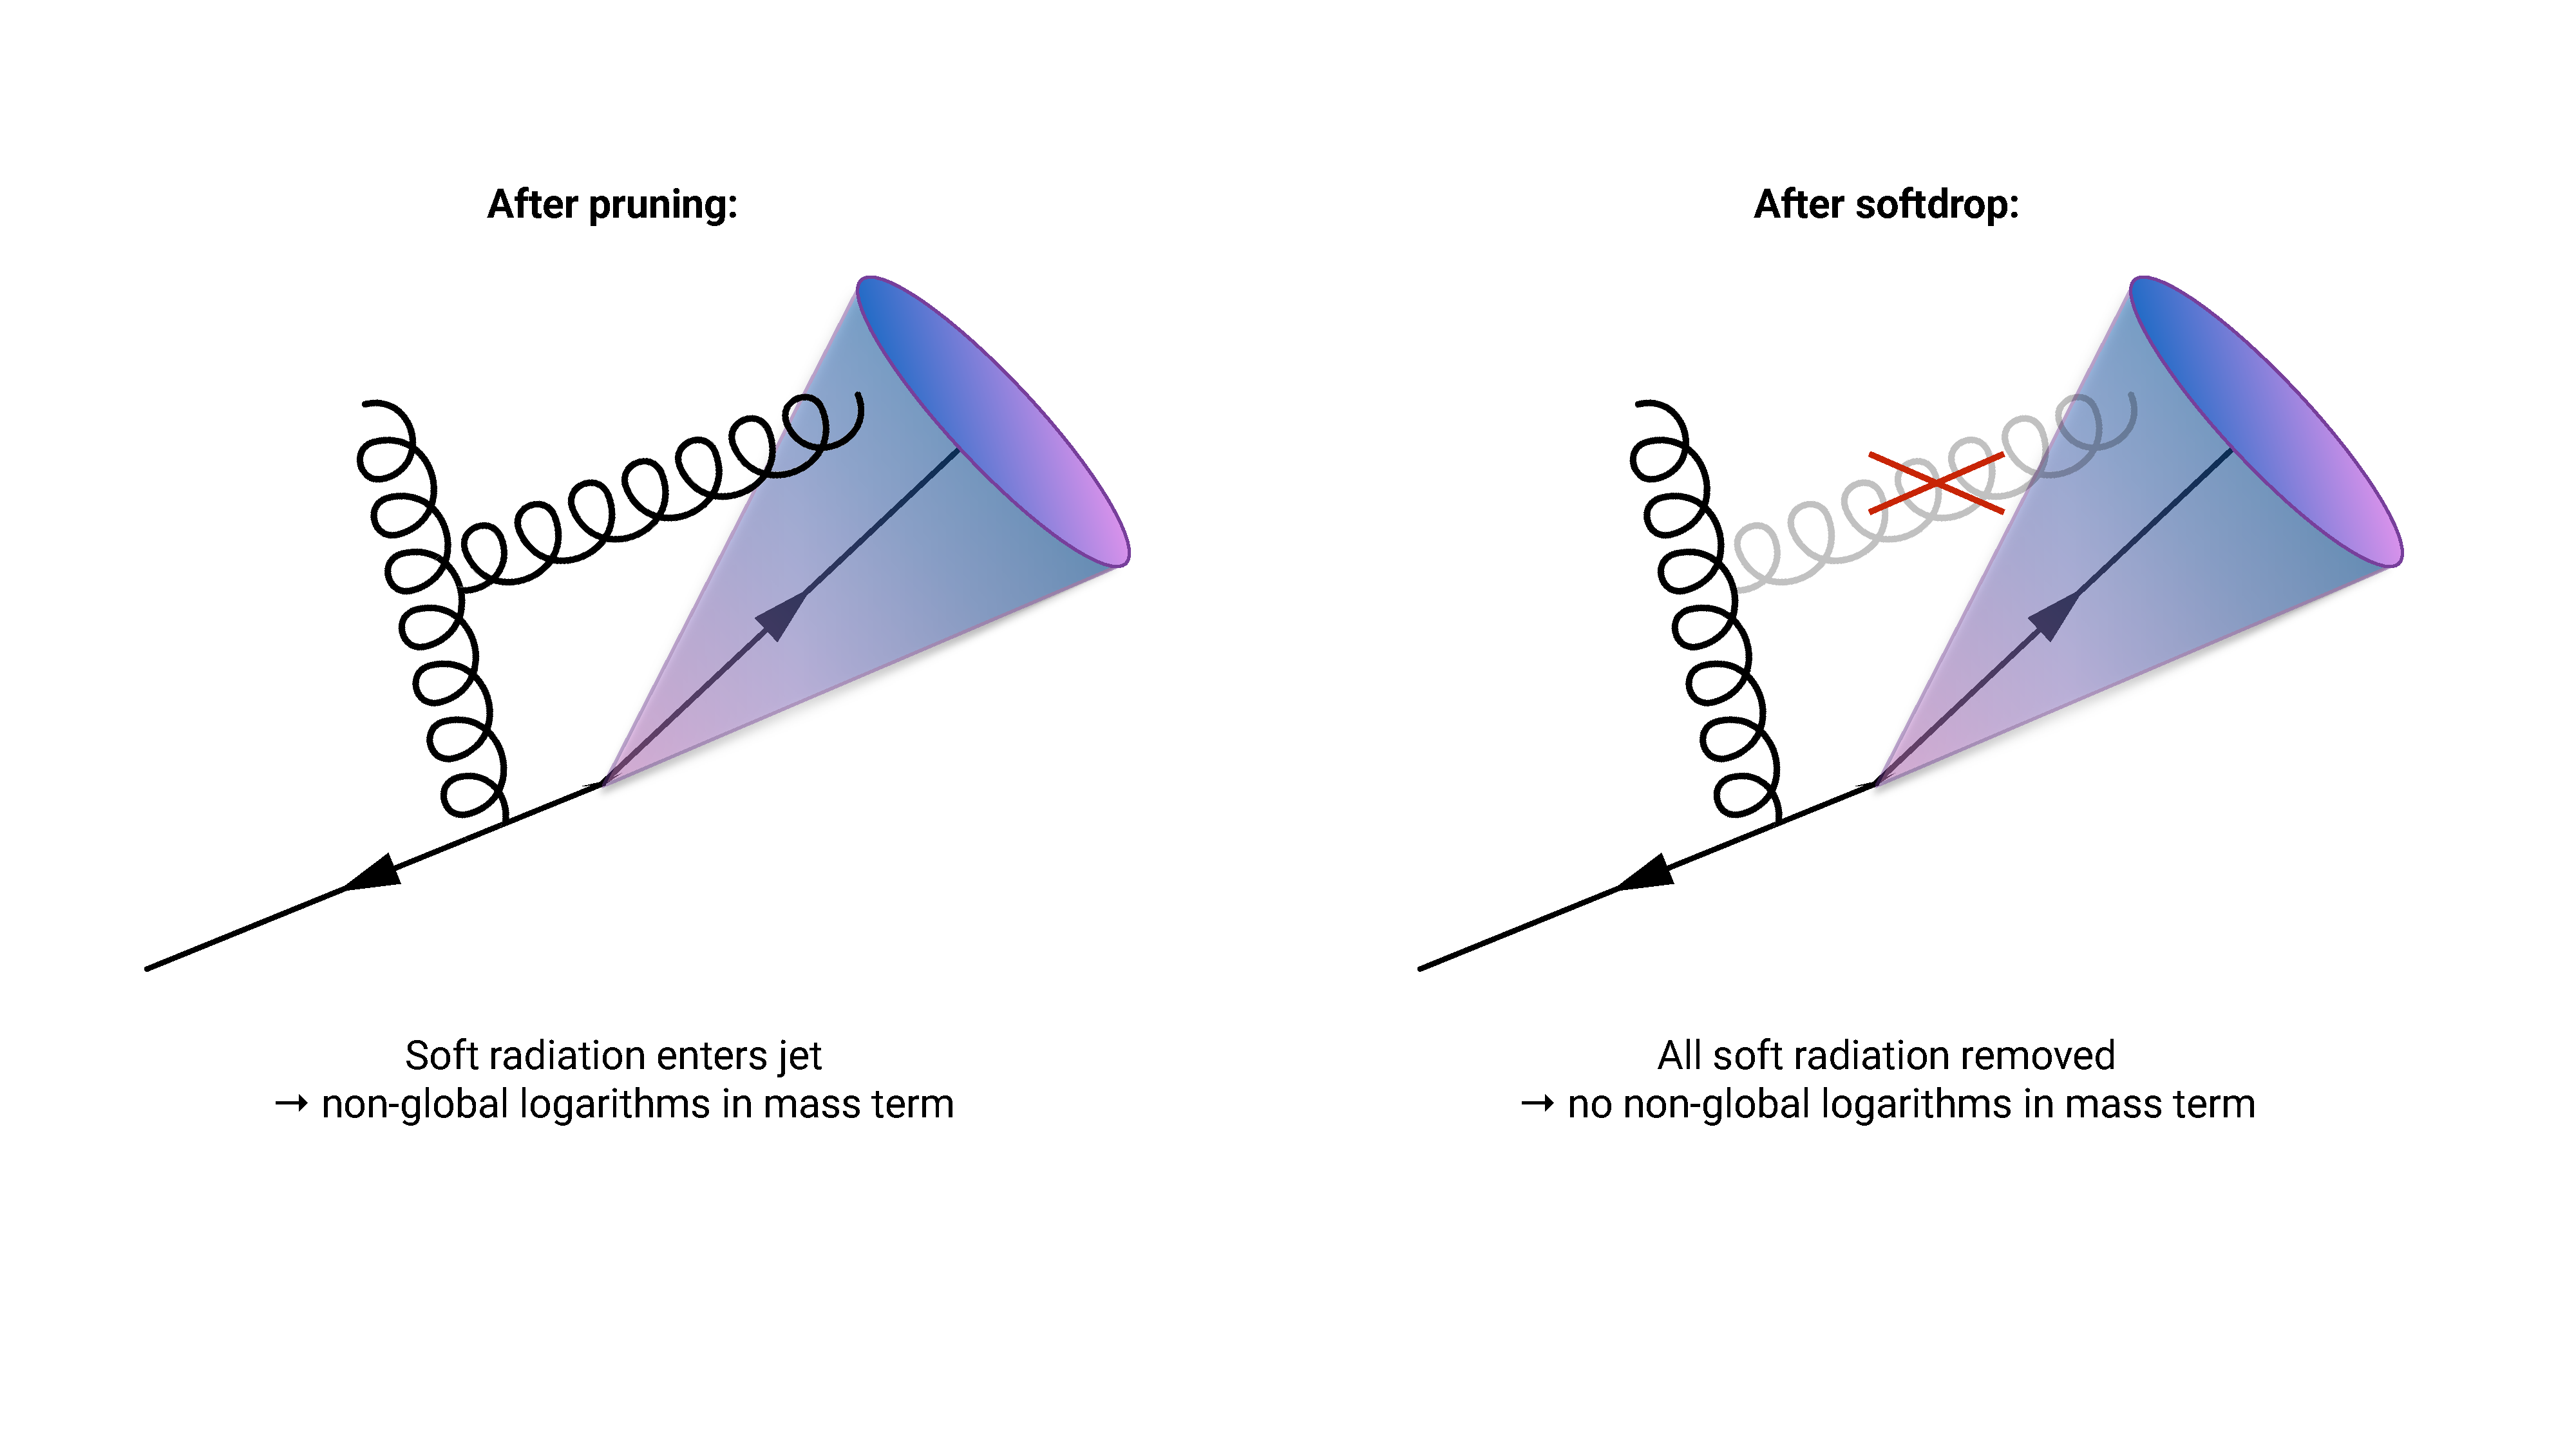
\includegraphics[width=0.69\textwidth]{figures/analysis/search2/misc/ngls.pdf}
\caption{The pruning algorithm does not remove all soft emission and therefore has non-global logarithmic terms in the jet mass. Softdrop ($\beta = 0$) completely removes soft emissions and is therefore free of non-global logarithms.}
\label{fig:searchII:ngls}
\end{figure}

The consequence of this is that you can calculate the softdrop jet mass to way higher precision than what is possible for other grooming algorithms or for the plain jet mass (NGLs are the main reason a full resummation of the plain jet mass beyond NLL (considering e.g multiple-emission effects) accuracy does not exist). Despite this not being a precision measurement analysis, we had theoretically well-motivated reasons for wanting the baseline CMS V-tagger to be softdrop-based. However, despite being less sensitive to soft radiation for QCD jets, signal jets groomed with softdrop were found to be far more sensitive to the underlying event than pruned jets~\cite{Dasgupta:2015yua}. Figure~\ref{fig:searchII:ue} shows the signal efficiency for pruning (left) and softdrop (right) as a function of jet transverse momenta when including FSR only, FSR+ISR, hadronization and hadronization + underlying event.


\begin{figure}[h!]
\centering
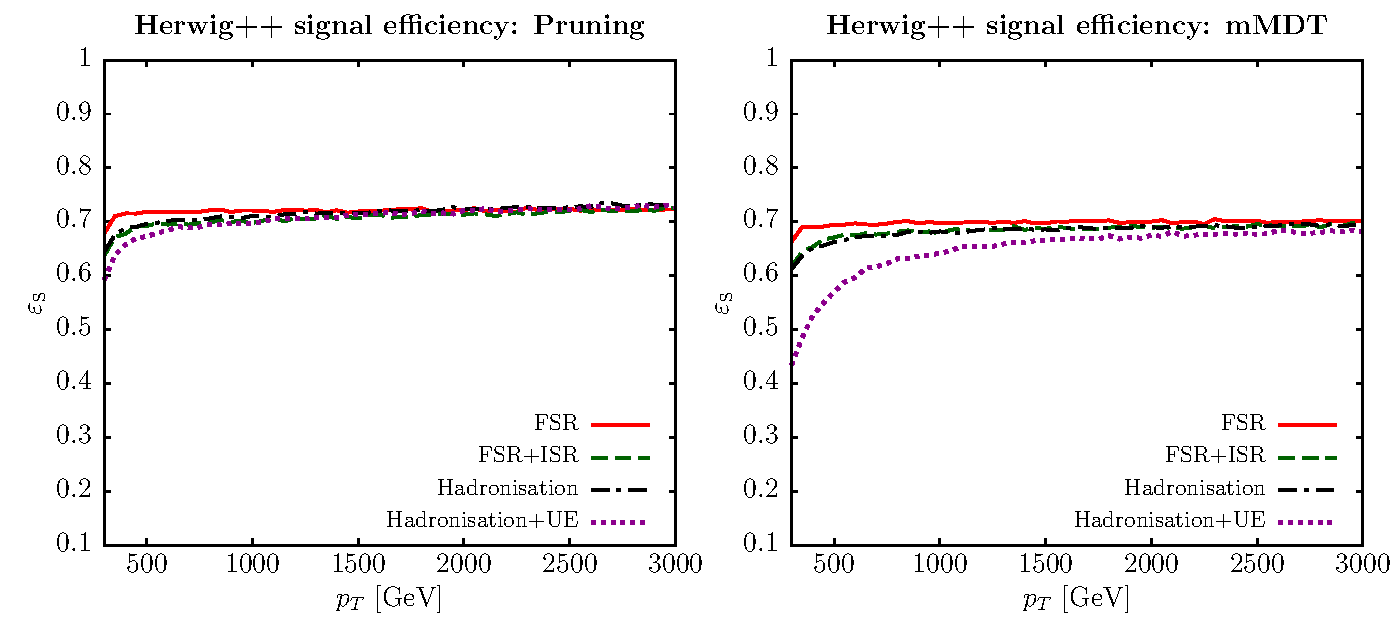
\includegraphics[width=0.79\textwidth]{figures/analysis/search2/misc/pruningvssd_ue.pdf}
\caption{The signal efficiency for pruning (left) and softdrop (right) as a function of jet \PT when adding FSR, ISR, hadronization and UE. THe UE has a severe impact on the softdrop efficiency for signal jets~\cite{Dasgupta:2015yua}. }
\label{fig:searchII:ue}
\end{figure}

On parton level, as well as after hadronization, the two algorithms perform very similar as a function of \PT. However, once UE contamination is added, the softdrop tagging efficiency is severely affected. This can be explained by the larger effective radius considered by the softdrop algorithm ( $\propto \mV/\PT \sqrt{z_{cut}(1-z_{cut})}$ ) in comparison to pruning ( $\propto \mV/\PT$ ). This observation corresponds very well with the shift in jet mass we observed for softdrop as a function of \PT in Section~\ref{sec:searchI:wtagging}: As the jet \PT decreases the softdrop effective radius increases and the jet mass mean shifts to higher values, due to absorbing more background radiation. If softdrop would be our new default tagger, a better rejection of pileup and UE contamination would be needed. In parallel to the ongoing theoretical work on groomers, a novel pileup removal algorithm had been proposed: Pileup per particle identification (PUPPI)~\cite{Bertolini2014}. Described in detail in Section~\ref{subsub:objreco:puppi}, PUPPI considers not only charged pileup but rather reweights each particle in the jet with its probability of arising from pileup. PUPPI had proven it self far superior to the current CHS algorithm in terms of jet mass resolution for large radius jets, and therefore seemed like the obvious choice to address both issues listed above: The sensitivity of softdrop regarding UE contamination and the strong pileup dependence of $\tau_{21}$. The focus of Search II would therefore be on the commissioning of a novel W-tagger, though there are interesting changes and inclusions in the analysis strategy as well: The inclusion of a $\PZpr \rightarrow \WW$ signal hypothesis and the addition of a completely new analysis, the single V-tag analysis.

\subsection{Analysis strategy}
The analysis strategy for this search is conceptually the same as for Search I. In addition, we'll take advantage of the n-subjettiness categorization and do an additional analysis in parallel: A search for excited quark resonances $\rm{q^*}$~\cite{Bauer1987,PhysRevD.42.815} decaying to qW or qZ.
We call this the single V-tag analysis, and the analysis selection only differs in that one jet is not required to pass the V-tag selection (groomed mass and n-subjettiness). The \VV analysis is hereby referred to as the double V-tag analysis. The difference between the two analyses is illustrated in Figure~\ref{fig:searchII:svsd}. 

\begin{figure}[h!]
\centering
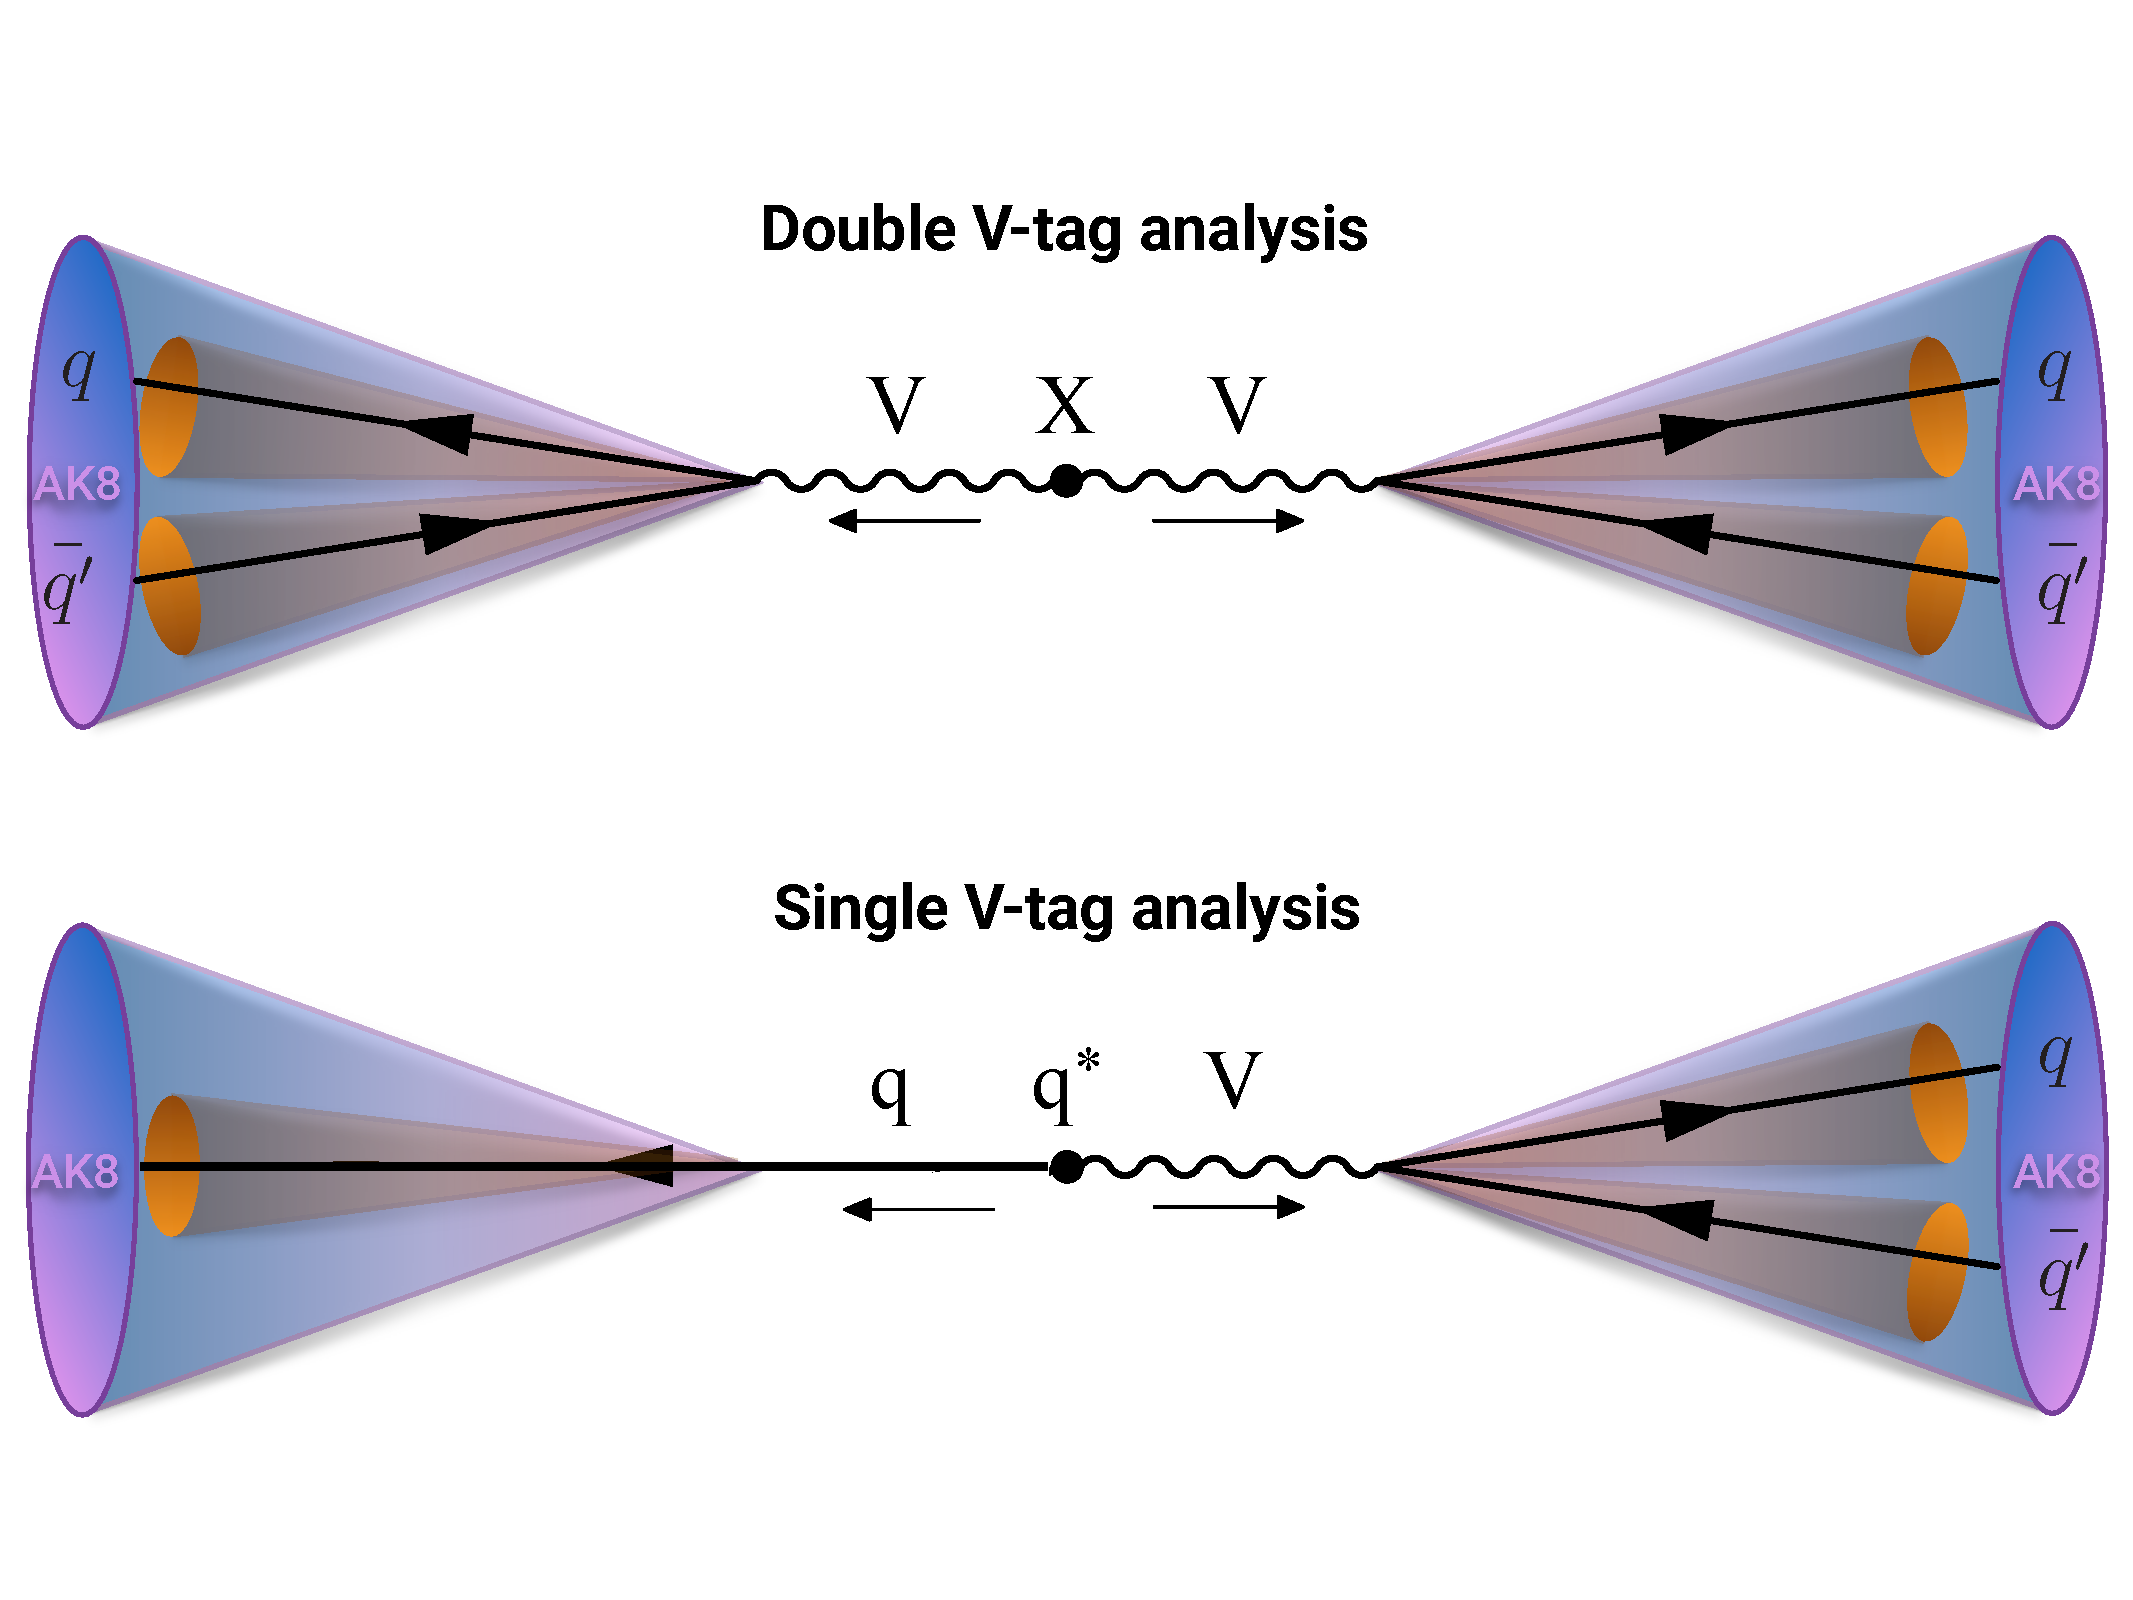
\includegraphics[height=6.5cm]{figures/analysis/search2/misc/singlevsdoubletag.pdf}
\caption{The double (top) and single (bottom) W/Z-tag analysis.}
\label{fig:searchII:svsd}
\end{figure}

In addition, limits are set on a $\PZpr \rightarrow \WW$ signal hypothesis in the double V-tag analysis, another 13 \TeV first.\newline
This analysis was published in two steps: An early Physics Analysis Summary based on 12.9 \fbinv of 2016 data~\cite{CMS-PAS-B2G-16-021}, describing the new  PUPPI+softdrop based V-tagger as well as the single V-tag analysis, and a second analysis topping up with the full 2016 data~\cite{PhysRevD.97.072006}. The commissioning of the new \PW\PZ-tagger has also been documented in a jet performance Physics Analysis Summary~\cite{CMS-PAS-JME-16-003}. I was 

\subsection{Data and simulated samples}
\label{sec:searchII:samples}
As mentioned above, the analysis of the 2016 dataset was done in two steps: One based on 12.9 \fbinv of early 2016 data describing the new W-tagger and single V-tag category, and a second topping up with the full 2016 dataset, corresponding to 35.9 \fbinv.\par
The \BulkG and HVT signal samples are modeled in precisely the same way as in 2015. For the single V-tag $\textrm{q}^*$ samples, we simulate unpolarized boson with a compositeness scale $\Lambda$ set equal to the resonance mass. These are generated to leading order using \PYTHIA version 8.212~\cite{Sjostrand:2007gs}. \par
The background Standard Model processes; QCD, W+jets and Z+jets are all simulated to leading order. V+jets is simulated with \amcatnlo~\cite{Alwall:2014hca,Alwall:2007fs}, while three different combinations of matrix element and shower generators is used for QCD as these predictions are known to differ: \PYTHIA only, the leading order mode of \amcatnlo{} matched with \PYTHIA, and \HERWIG{++}~2.7.1~\cite{Bahr:2008pv} with tune CUETHS1~\cite{Khachatryan:2015pea}.

\subsection{Event selection}

\subsubsection{Triggering}

The triggers used in this analysis are the same ones as in 2015 (see Section~\ref{sec:search1:trigger}), however, due to the new single V-tag analysis, the trigger turn-ons have this time been re-evaluated separately requiring either one or two jets to have an offline softdrop jet mass above 65 \GeV.
\par Figure~\ref{fig:searchII:trigger-fits} shows the trigger turn-on curves as a function of dijet invariant mass for jets passing one of the three inclusive triggers only, one of the grooming triggers only and when combining all of them. The turn-on curves are shown for all jet pairs passing loose selections as described in Section \ref{sec:search1:preselection}. Zero, one or two of the two jets is further required to have a softdrop mass larger than 65 GeV.

\begin{figure}[h!]
\centering
% 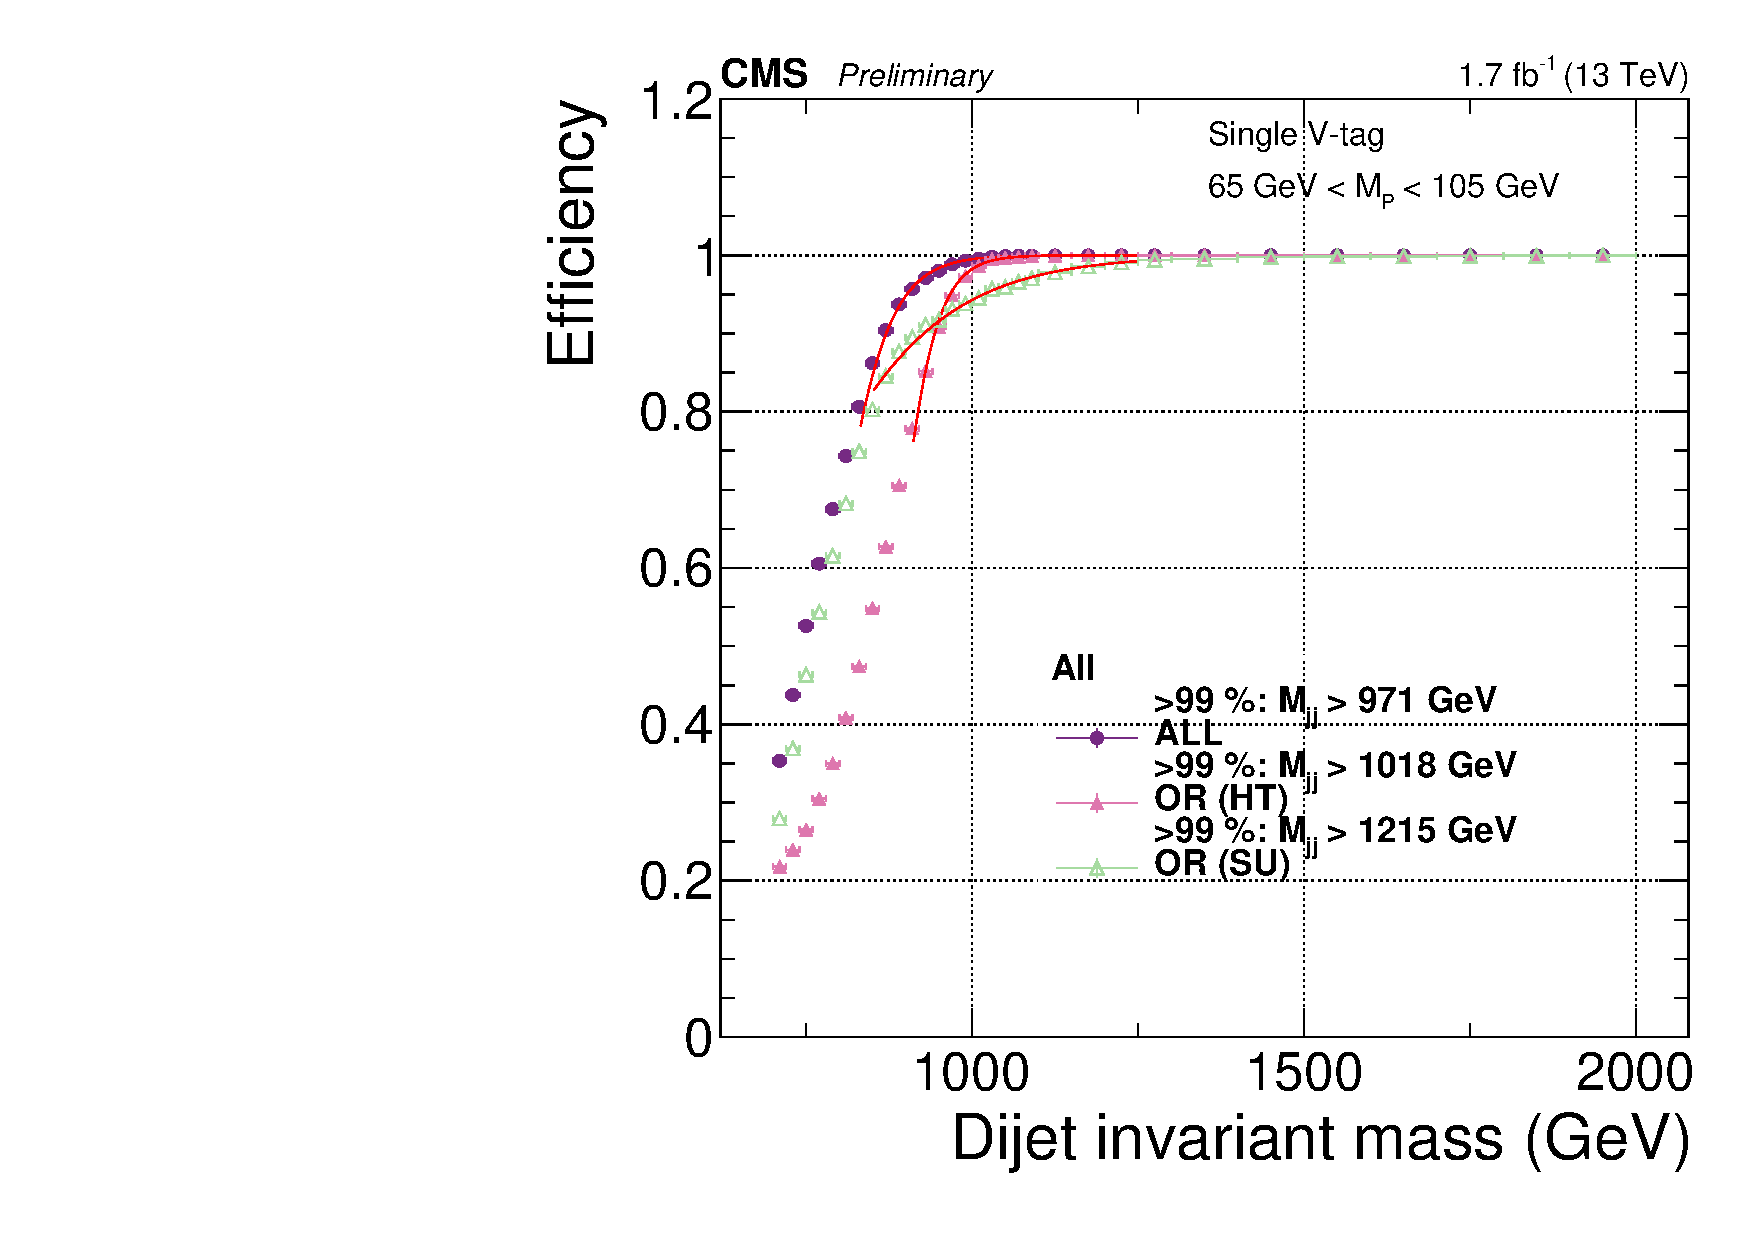
\includegraphics[width=0.4\textwidth]{figures/analysis/search2/AN-16-398/plots/trigger/triggereffMjj-ALL_SingleTag_runAll.pdf}
% 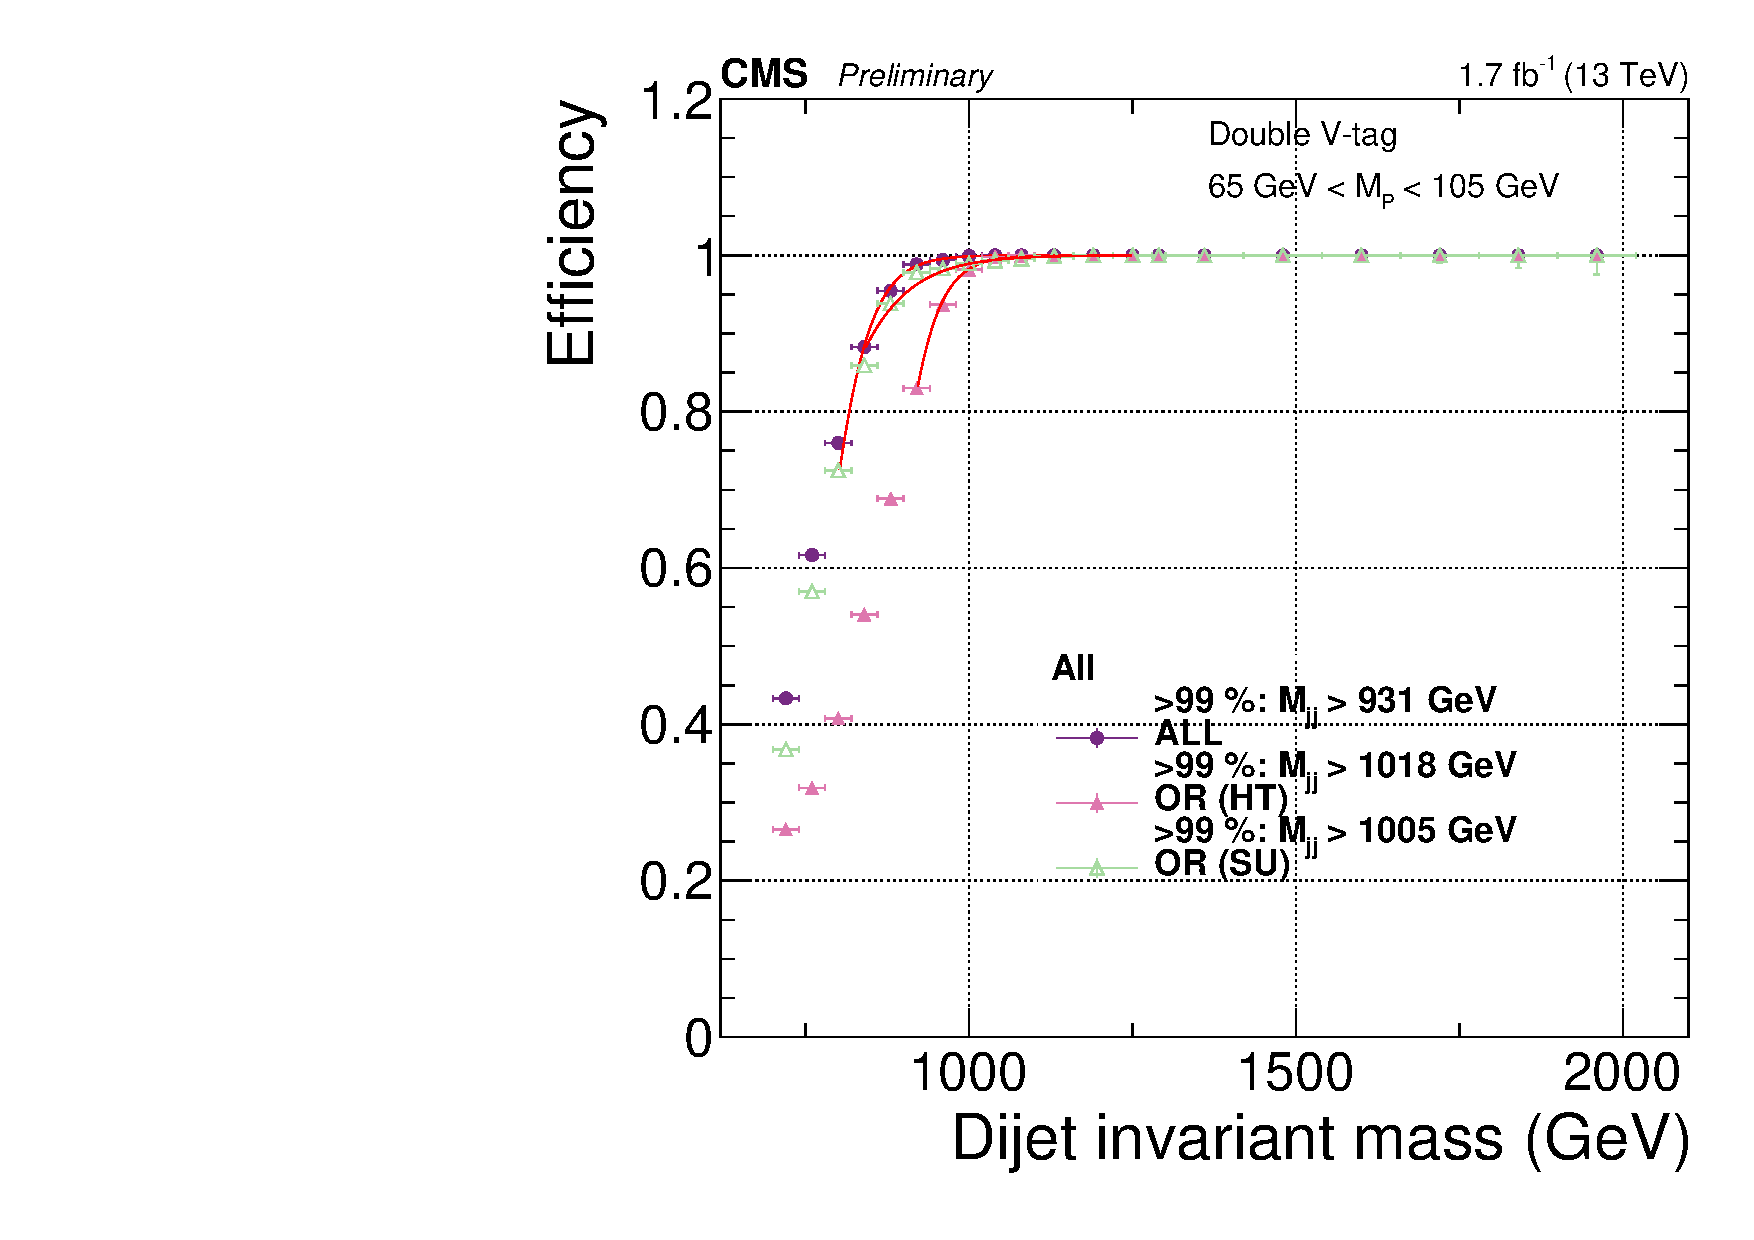
\includegraphics[width=0.4\textwidth]{figures/analysis/search2/AN-16-398/plots/trigger/triggereffMjj-ALL_DoubleTag_runAll.pdf}
% 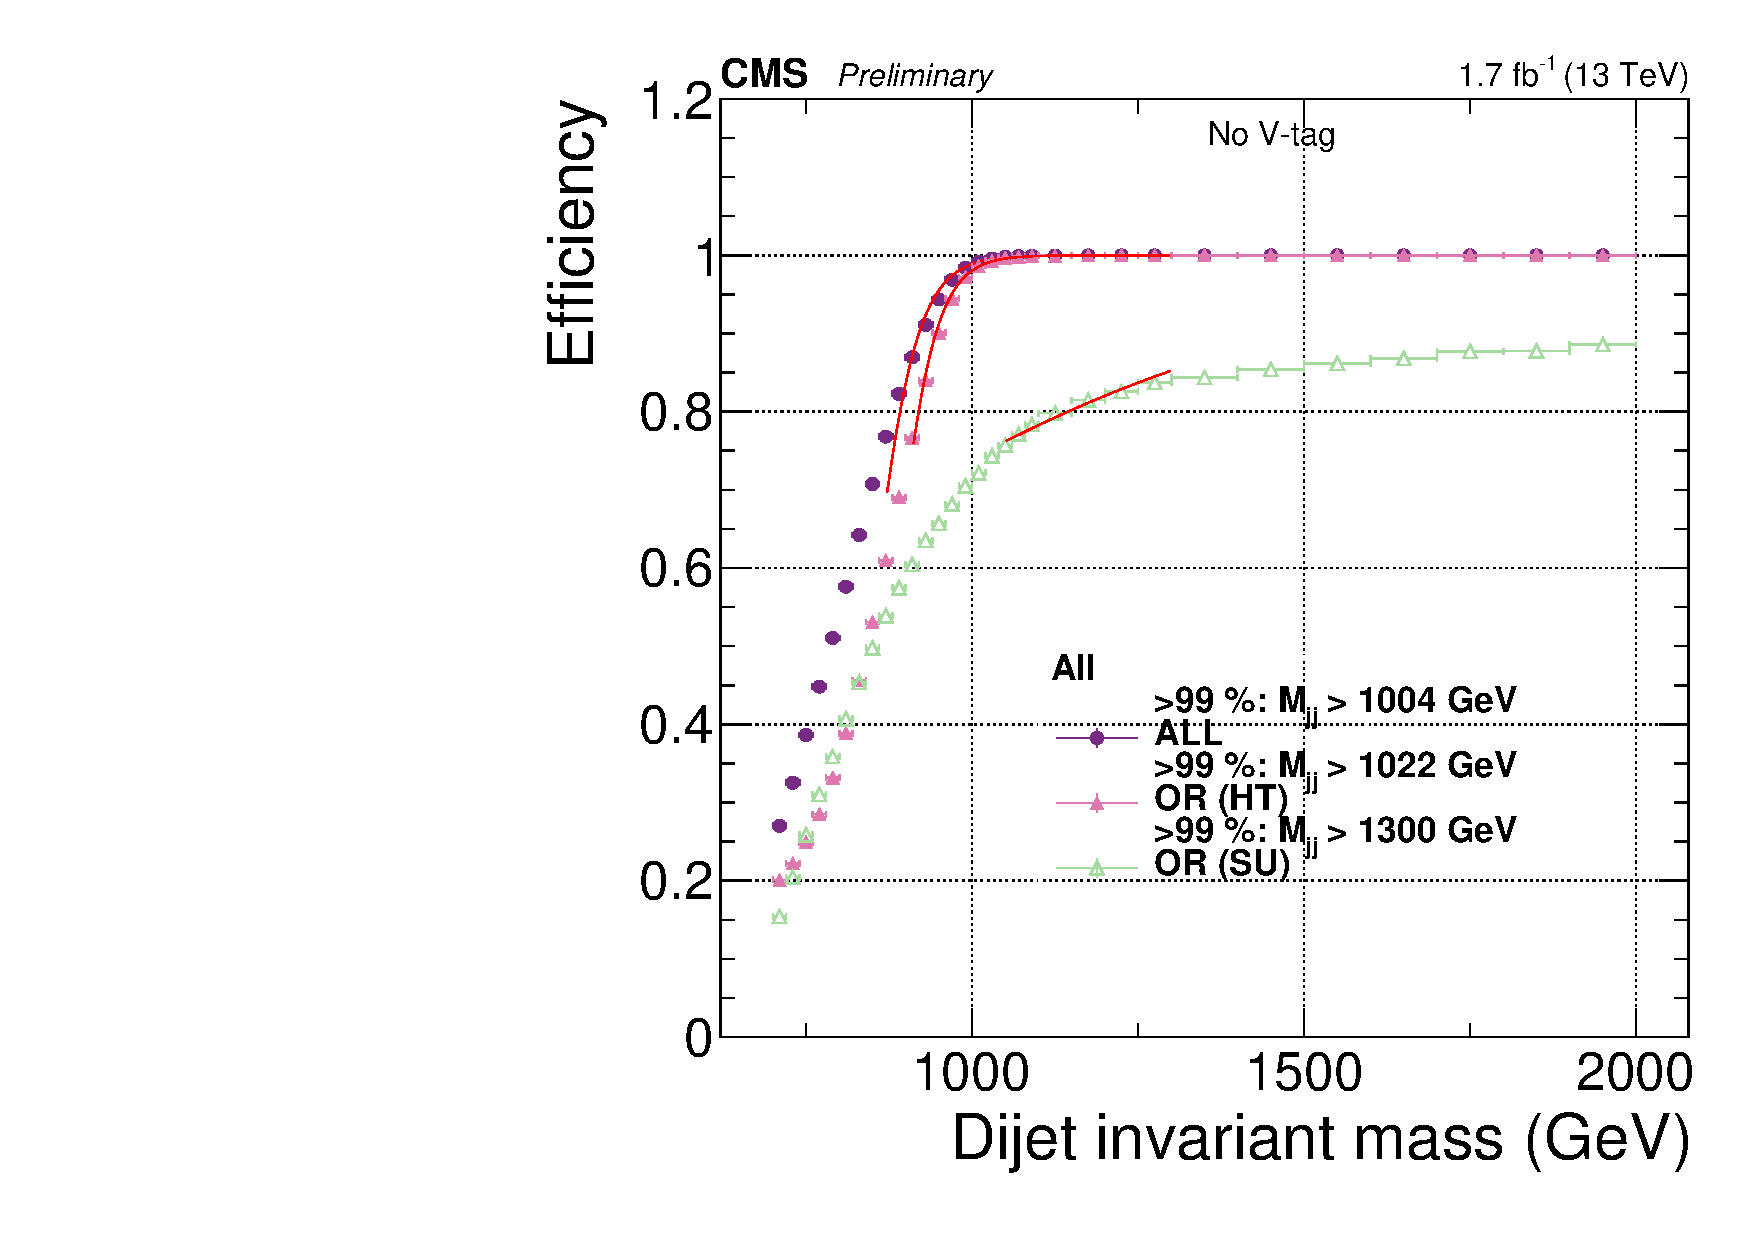
\includegraphics[width=0.4\textwidth]{figures/analysis/search2/AN-16-398/plots/trigger/triggereffMjj-ALL_noTag_runAll.pdf}
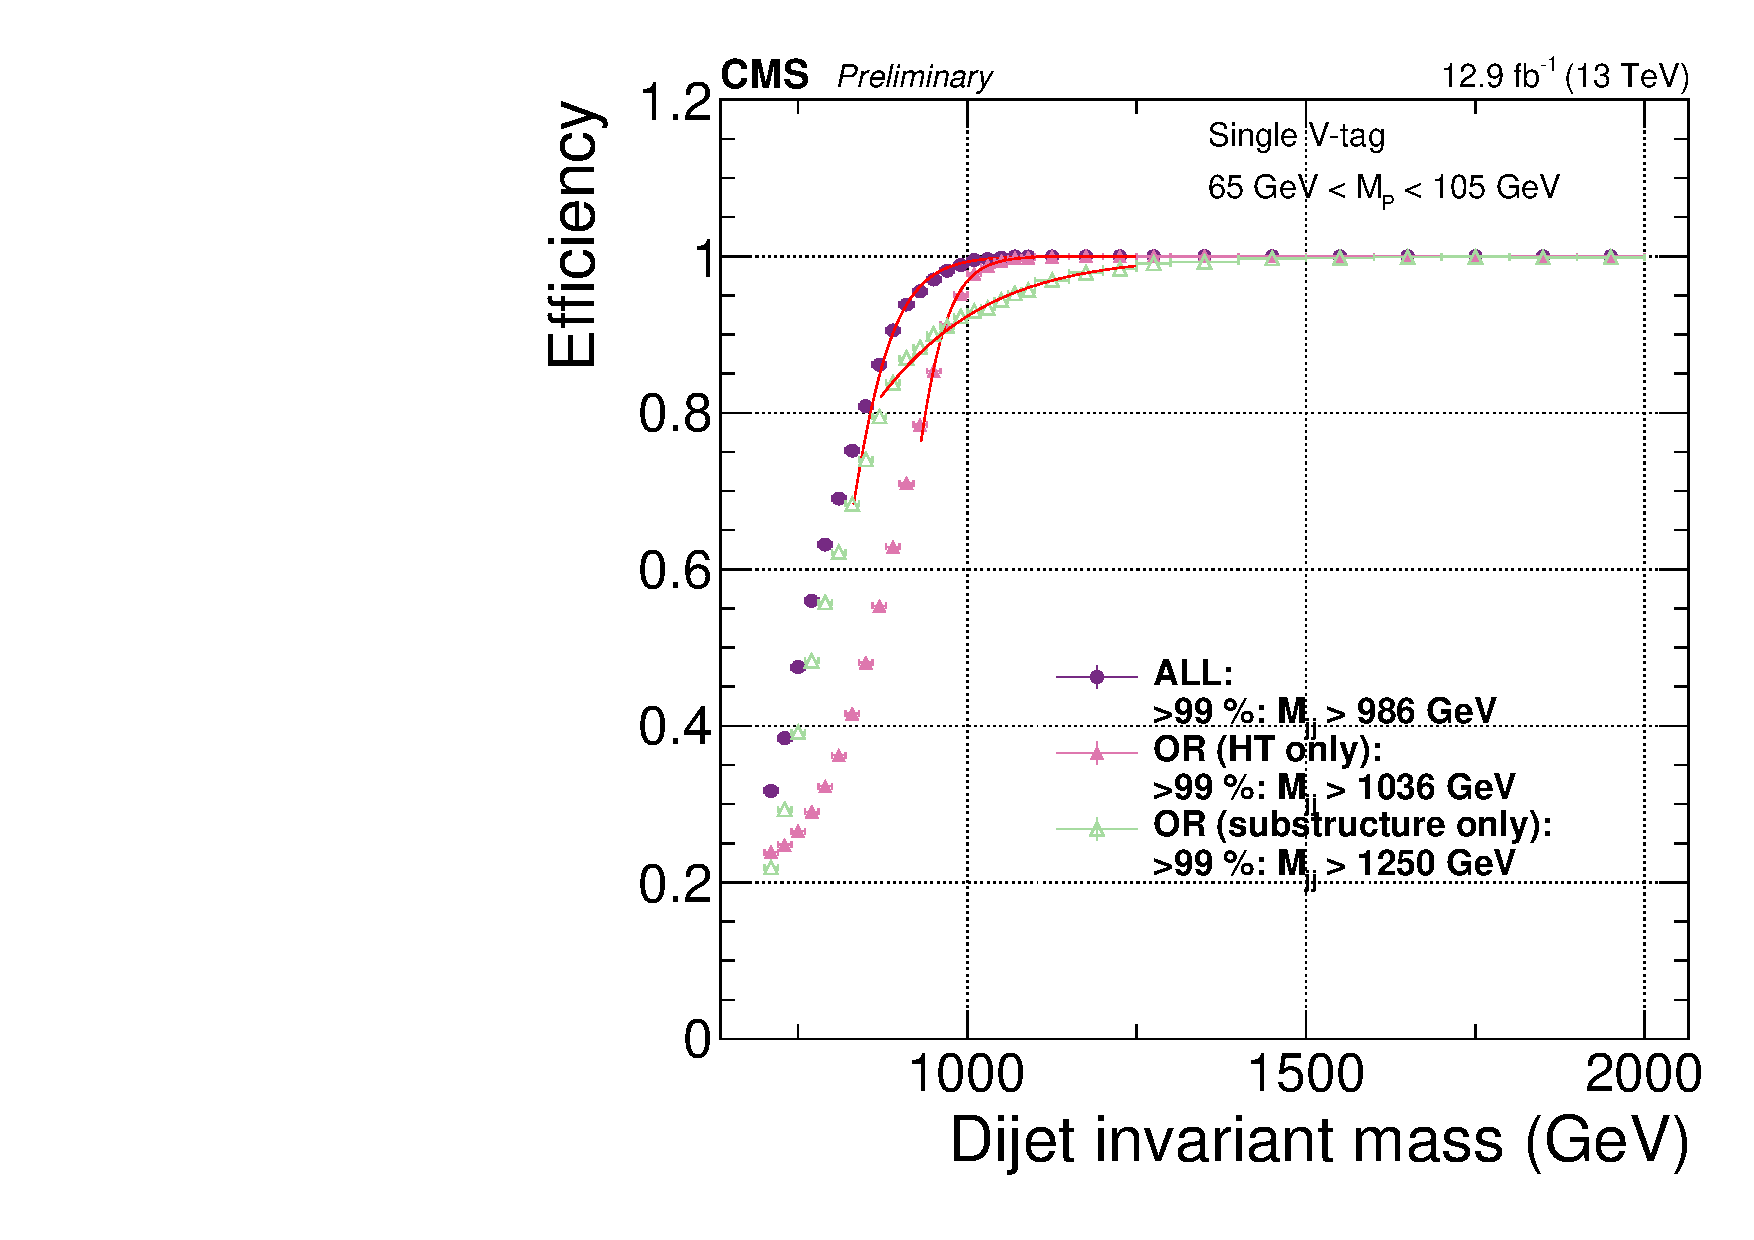
\includegraphics[width=0.4\textwidth]{figures/analysis/search2/AN-16-235/plots/triggereffMjj-ALL_SingleTag.pdf}
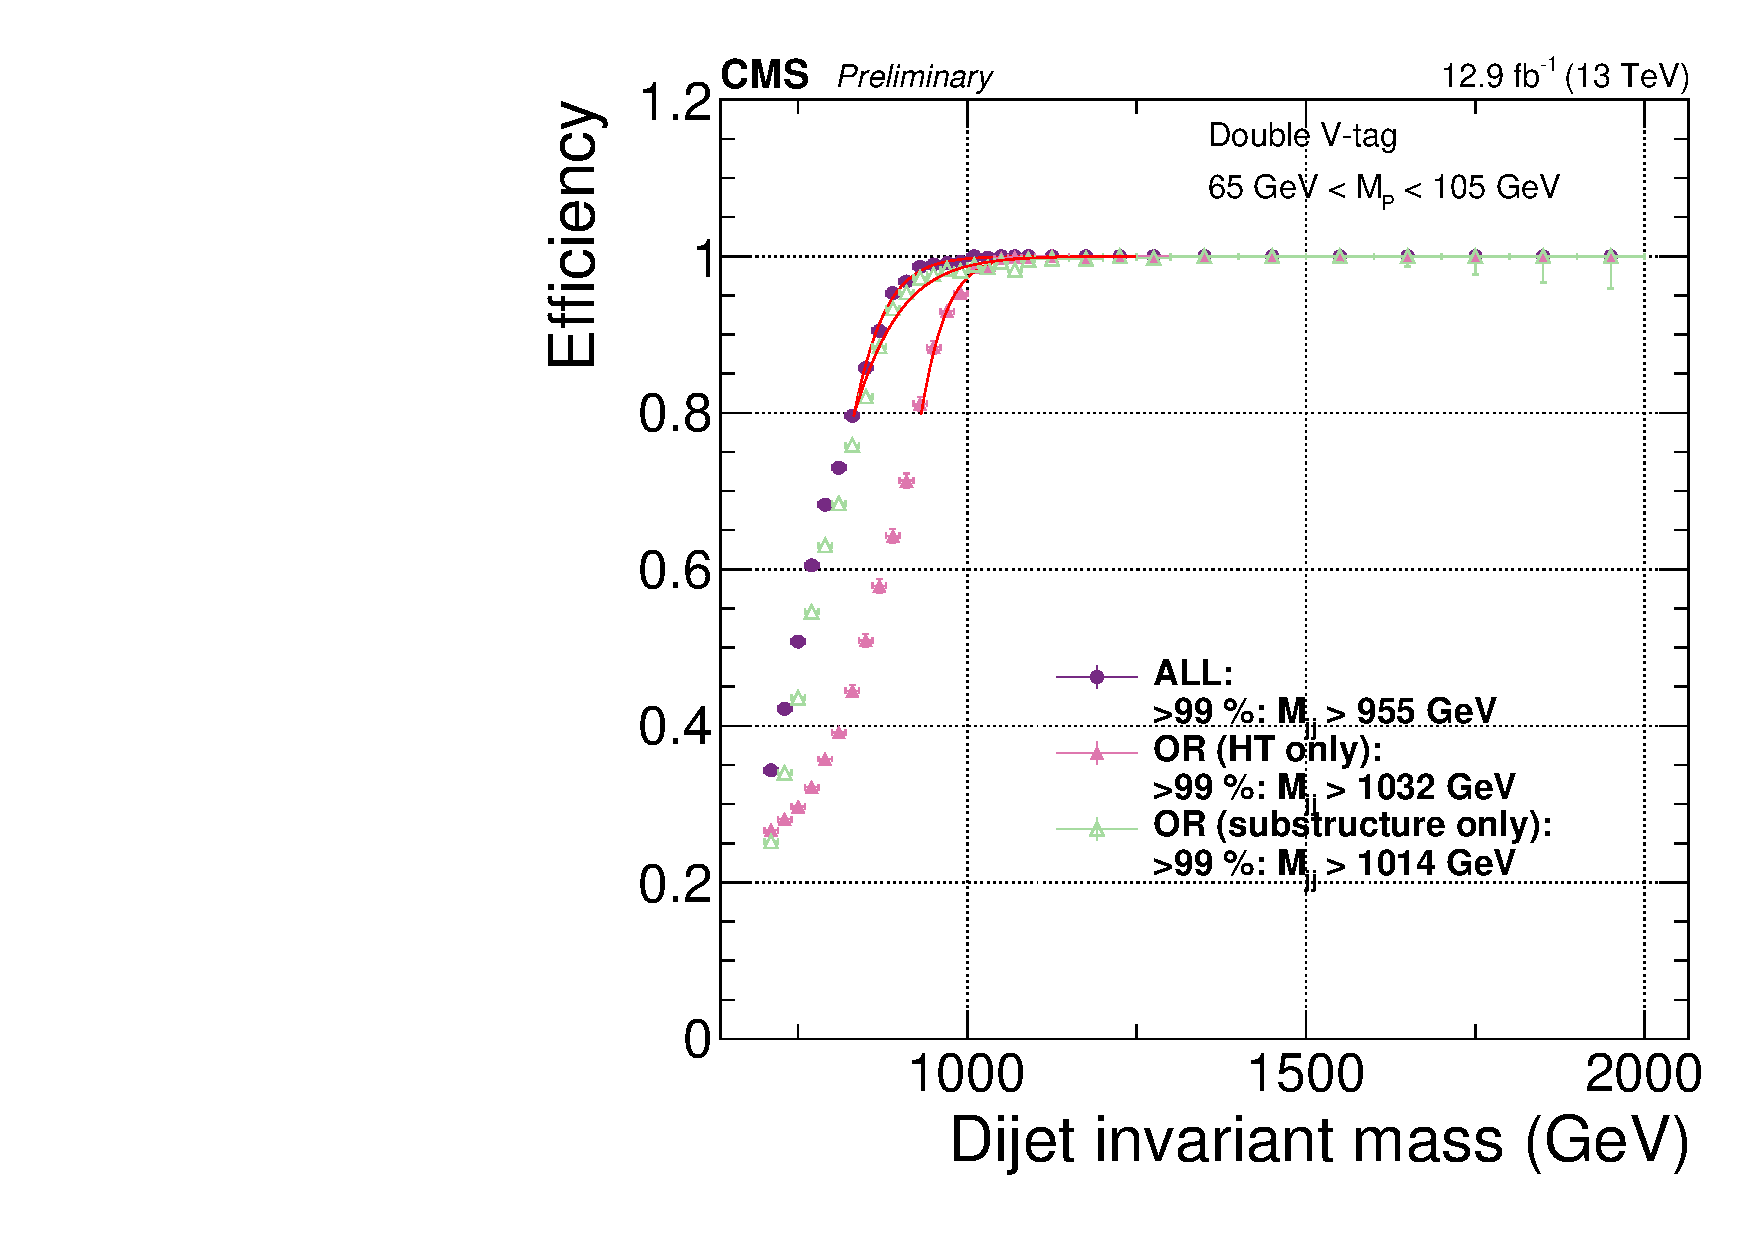
\includegraphics[width=0.4\textwidth]{figures/analysis/search2/AN-16-235/plots/triggereffMjj-ALL_DoubleTag.pdf}\\
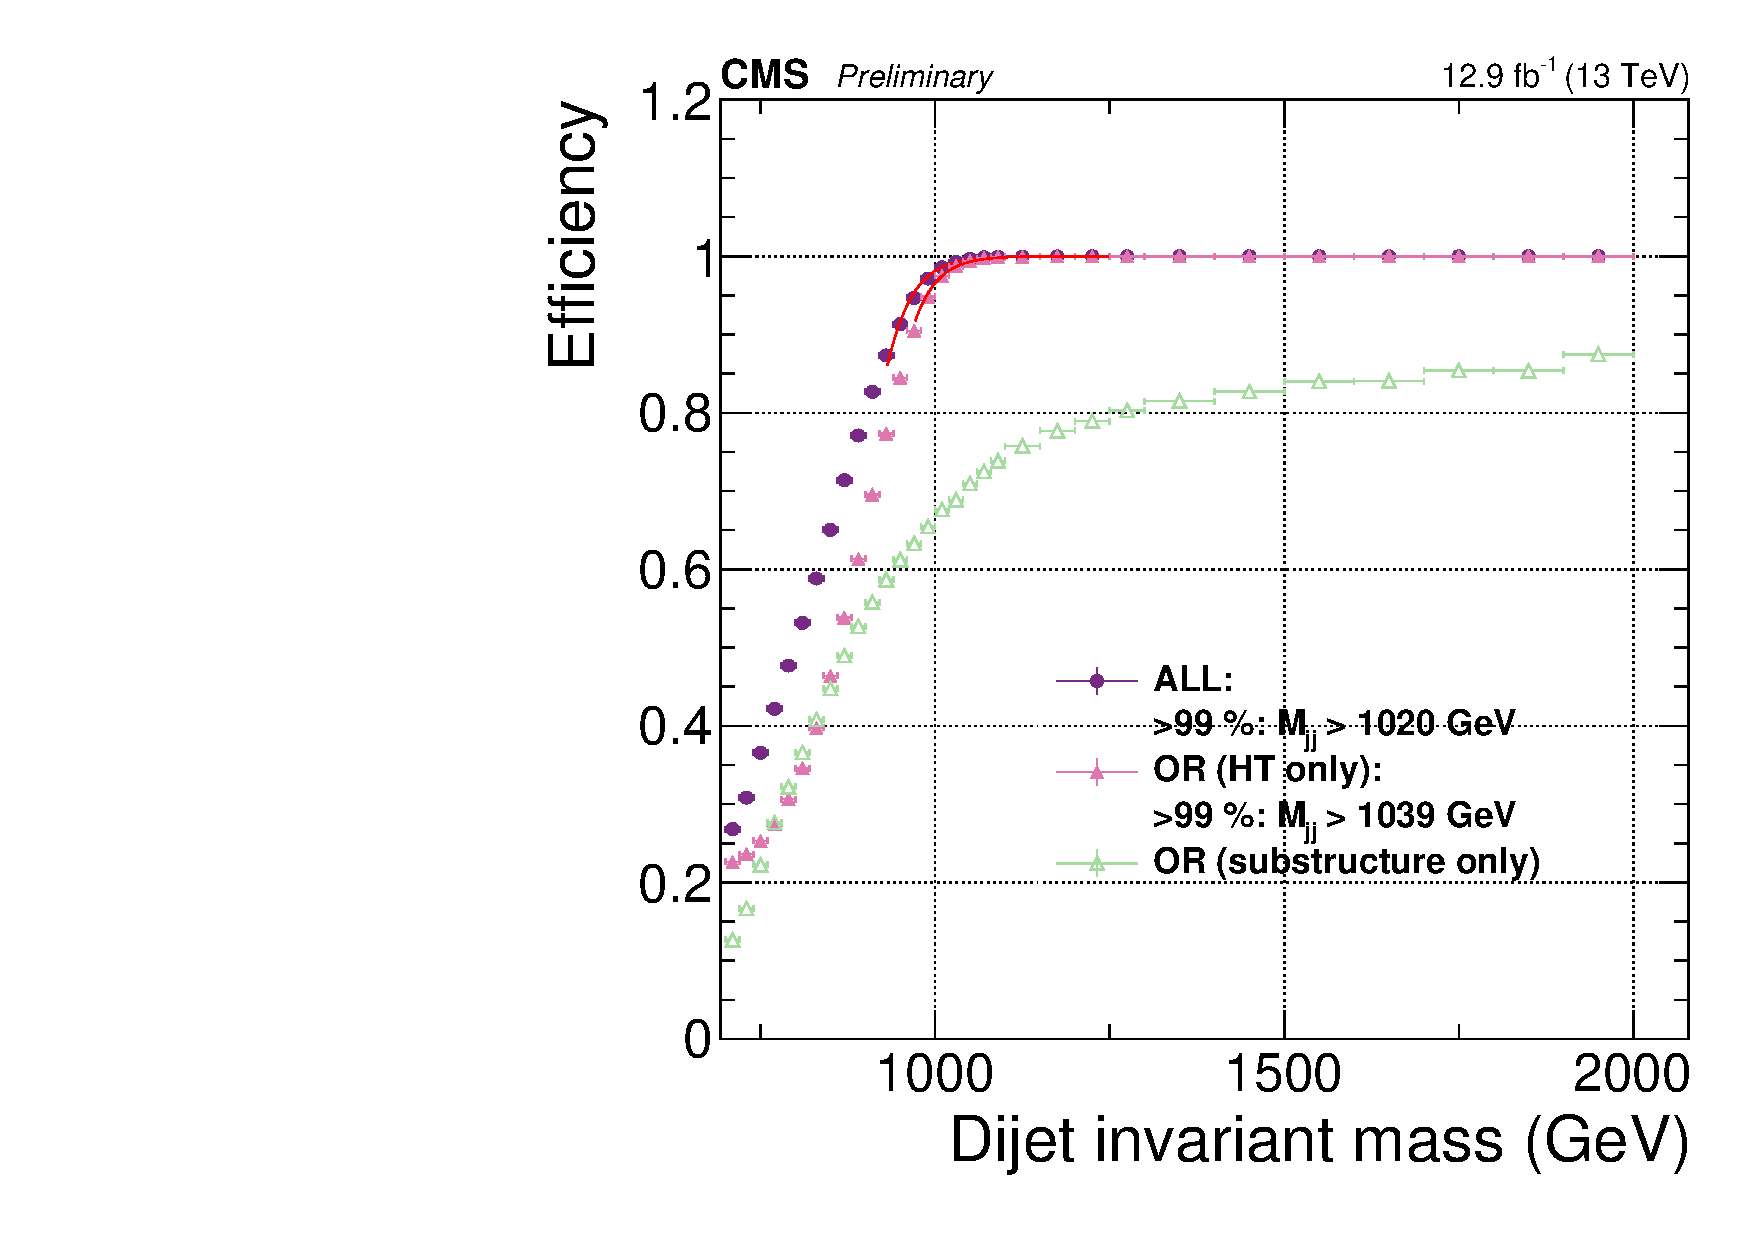
\includegraphics[width=0.4\textwidth]{figures/analysis/search2/AN-16-235/plots/triggereffMjj-ALL_noTag.pdf}

\caption{Comparison of trigger efficiencies for jets passing one of the HT-triggers only (pink), for jets passing one of the grooming-triggers only (green) and for jets passing one of the HT-triggers or one of the grooming triggers (purple). Here as a function of dijet invariant mass for all jet pairs passing loose selections and where one jet has a softdrop mass larger than 65 GeV (top left), both jets have a softdrop mass larger than 65 GeV (top right) and where no mass cut is applied (bottom). }
\label{fig:searchII:trigger-fits}
\end{figure}

Including grooming triggers lowers the 99\% trigger efficiency threshold by around 50(80) \GeV in the single (double) tag category once substructure is requested on the analysis level. Using the or of all triggers, we are safely on the trigger plateau for dijet invariant masses above 955(986) \GeV in the double (single) tag category, setting the analysis threshold at a dijet invariant mass of 955 \GeV for the double tag analysis and 990 \GeV for the single tag analysis. For controlplots where no groomed mass window is applied, a trigger threshold of 1020 GeV is used.

\par Trigger efficiencies as a function of the offline softdrop-jet mass for the \\ 
\texttt{HLT\_AK8PFJet360\_TrimMass30} trigger are shown in Figure~\ref{fig:searchII:grooming-mj-trigger}. Here the jet transverse momentum of one of the jets is required to be at least 600 GeV and no other mass cut is applied. This trigger requires one jet to have a trimmed mass above 30 GeV at HLT level and reaches the trigger plateau for groomed-jet masses around 50 GeV. As reference trigger, the prescaled trigger \texttt{HLT\_PFJet320} is used. 
\begin{figure}[htb]
\centering
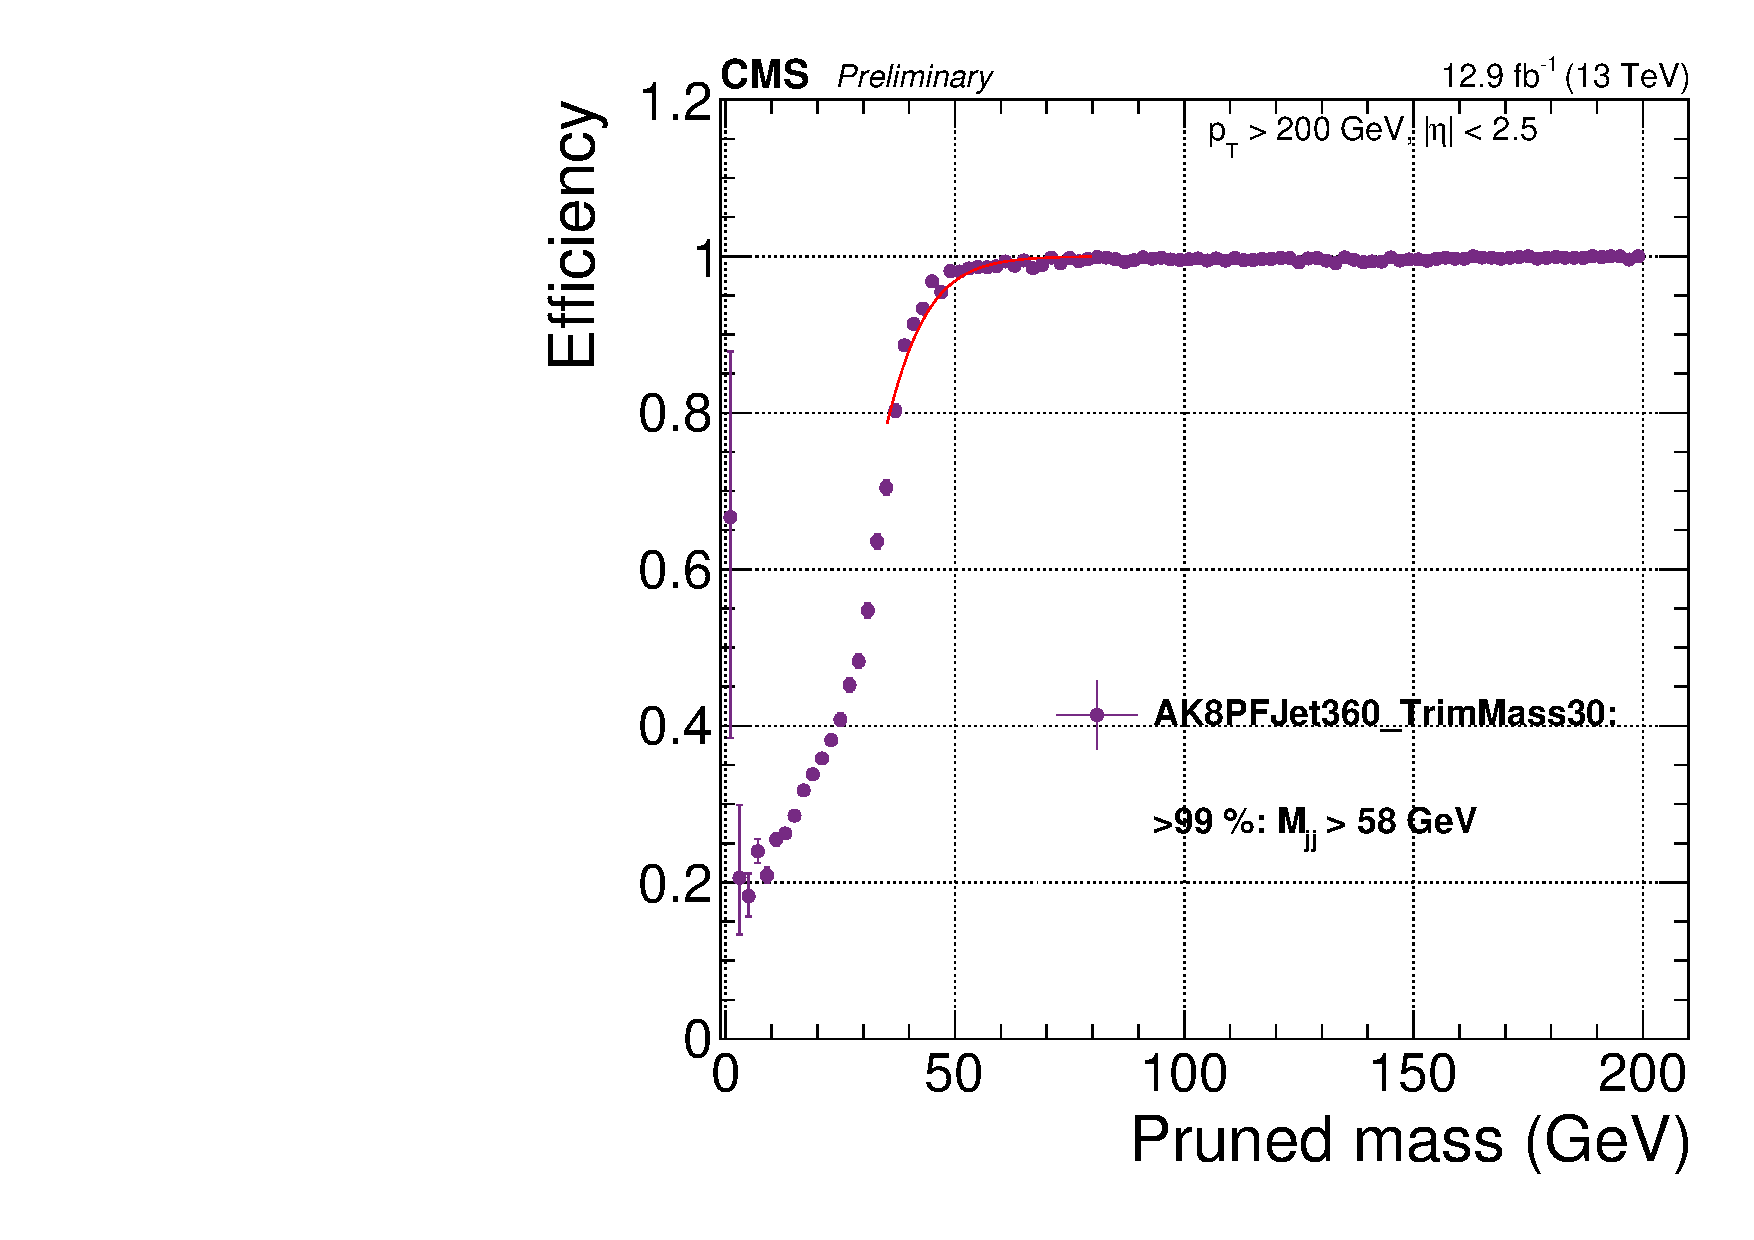
\includegraphics[width=0.4\textwidth]{figures/analysis/search2/AN-16-235/plots//triggereff-prunedmass_fit.pdf}
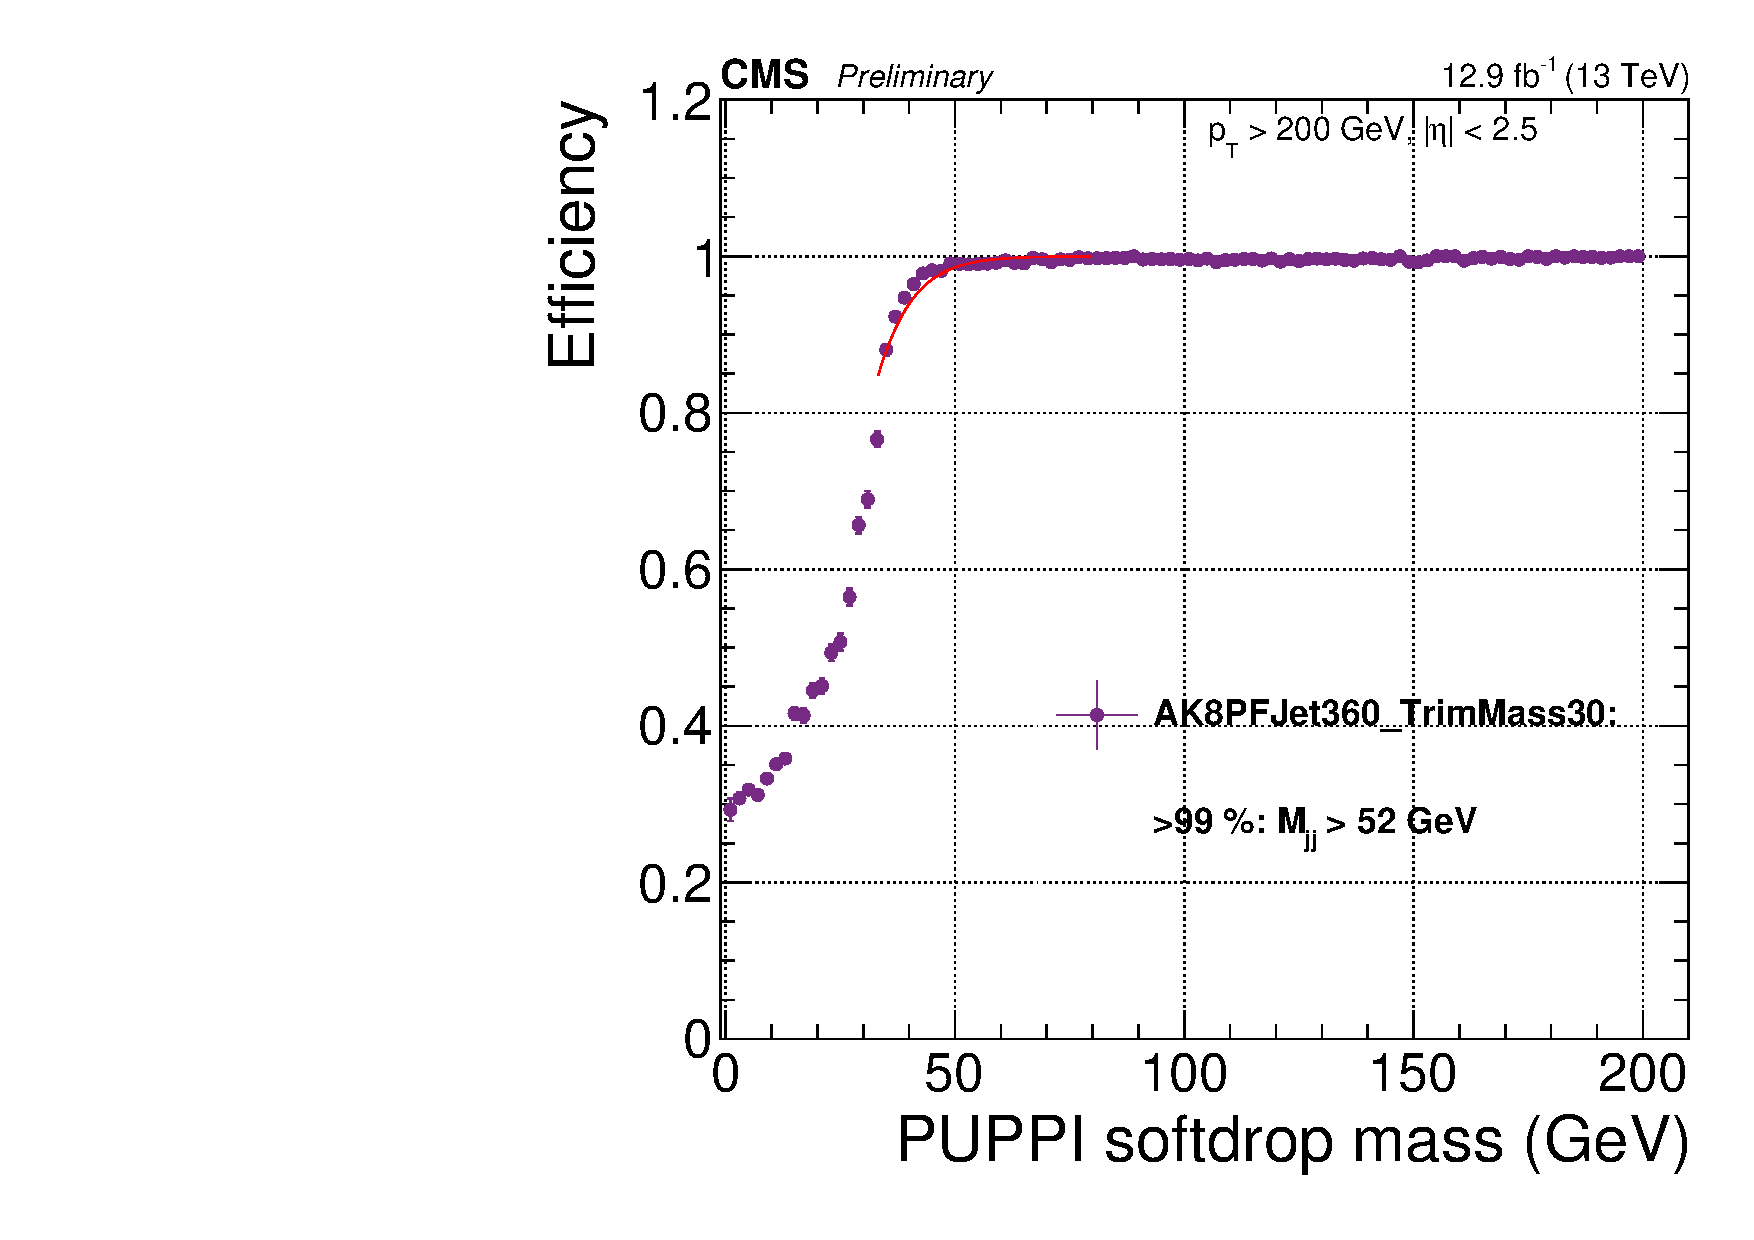
\includegraphics[width=0.4\textwidth]{figures/analysis/search2/AN-16-235/plots//triggereff-sdmass_fit.pdf}
\caption{Efficiency for the \texttt{HLT\_AK8PFJet360\_TrimMass30} trigger as a function of pruned-jet (left) and softdrop-jet (right) mass for jets with $\PT > \unit{600}{\GeV}$.}
\label{fig:searchII:grooming-mj-trigger}
\end{figure}



\subsection{Developing a new W-tagger}
\label{sec:searchII:puppisoftdrop}